\documentclass[logo,reportComp]{thesis}
\usepackage[cpp,pseudo]{mypackage}

\title{高级编程技术实验报告}
\subtitle{实验五:模拟全球变暖}
\school{数据科学与计算机学院}
\author{陈鸿峥}
\classname{17大数据与人工智能}
\stunum{17341015}
\headercontext{高级编程技术实验报告}
\lstset{language=python}

\begin{document}

\maketitle

\section{问题描述、求解思路及实验结果}
\subsection*{Part A:创建模型}
\subsubsection{曲线拟合}
\verb'generate_models':直接将\verb'pylab.polyfit(x,y,deg)'的结果添加入结果列表中即可

\subsubsection{计算$R^2$}
依照公式
\[R^2=1-\frac{\sum_{i=1}^n(y_i-e_i)^2}{\sum_{i=1}^n(y_i-\text{mean})^2}\]
对应进行计算即可,注意这里用到了类numpy的向量运算
\begin{lstlisting}
def r_squared(y, estimated):
    mean = sum(y) / len(y)
    numerator = sum((y - estimated)**2)
    denominator = sum((y - mean)**2)
    return 1 - numerator / denominator
\end{lstlisting}

\subsubsection{模型可视化}
\verb'evaluate_models_on_training'的实施过程如下
\begin{itemize}
	\item 枚举\verb'models'中的每一个模型
	\item 创建估计值数组:\verb'estimated = pylab.zeros(len(x))'
	\item 利用Python数组的负数索引,还原出拟合模型的多项式表达式,通过不断累加得到估计值,注意这里同样是进行向量运算
\begin{lstlisting}
for i in range(len(model)):
    estimated += model[-i-1] * x**i
\end{lstlisting}
	\item 计算\verb'r_squared'和\verb'se_over_slope'
	\item 利用\verb'plot'函数画图,同时利用\verb'xlabel'、\verb'ylabel'和\verb'title'对图像进行标识
\end{itemize}

\subsubsection{调查趋势}
依照题目要求,先从\verb'climate'中获取必要的日/年份信息,然后用\verb'generate_models'生成模型,再用\verb'evaluate_models_on_training'进行模型评估。

注意对于年温度来说,需要对该年所有气温求均值,该年是否为闰年需要小心判断。
代码细节如下。
\begin{lstlisting}
climate = Climate("data.csv")
years = pylab.array(TRAINING_INTERVAL)

# Part A.4
# I. January 10th
temperature = [climate.get_daily_temp("NEW YORK",1,10,year) for year in years]
temperature = pylab.array(temperature)
model = generate_models(years,temperature,[1])
evaluate_models_on_training(years,temperature,model)

# II. Annual Temperature
temperature = []
for year in years:
    yearly_temp = pylab.sum(climate.get_yearly_temp("NEW YORK",year))
    temperature.append(yearly_temp / (366 if (year % 4 == 0 and year % 100 != 0) or (year % 400 == 0) else 365))
temperature = pylab.array(temperature)
model = generate_models(years,temperature,[1])
evaluate_models_on_training(years,temperature,model)
\end{lstlisting}

\begin{figure}[H]
\centering
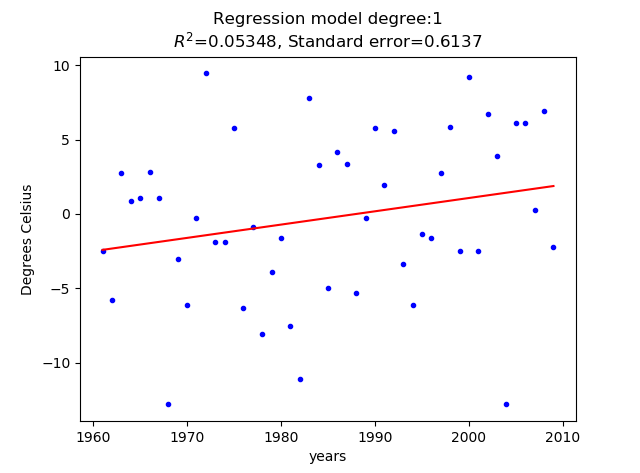
\includegraphics[width=0.6\linewidth]{fig/4I.png}
\caption{问题4.I结果}
\end{figure}
\begin{figure}[H]
\centering
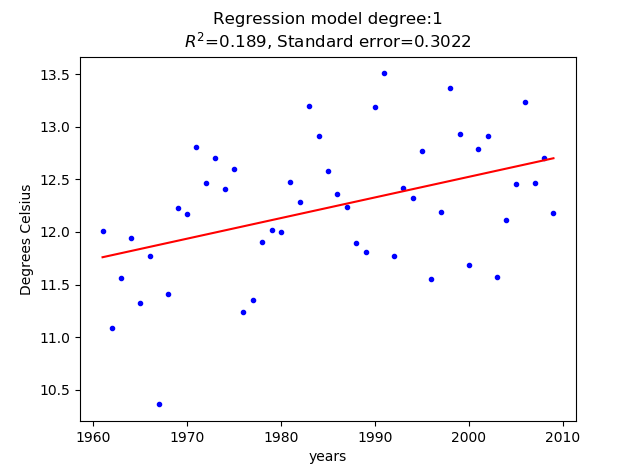
\includegraphics[width=0.6\linewidth]{fig/4II.png}
\caption{问题4.II结果}
\end{figure}

Writeup回答
\begin{itemize}
	\item 日气温的$R^2$更小,但年气温的拟合效果更好(这可能是因为噪声少导致的,见下题)。
	不管是日气温还是年气温$R^2$都远小于$0.5$,故气温上升趋势的显著性非常大。
	\item 因为每日/每年的气温具有随机性,因此噪声非常多。
	日气温的噪声更严重,因为日与日之间的差异很可能很大,而一整年的气温平均下来可以一定程度上消除噪声。
	\item 问题一已经回答,从图中确实可以看出气候在变暖。
	红色上升的拟合线及非常小的$R^2$都证实了气温上升,且可信度很高,标准误差都在$0.5$摄氏度左右。
\end{itemize}

\subsection*{Part B:处理更多数据}
\verb'gen_cities_avg'要注意遍历的方式及求平均的对象。
本题中应该对某一城市某一特定年份的所有天数气温求平均后,再对该年所有城市的平均气温求平均,如下代码所示。
\begin{lstlisting}
def gen_cities_avg(climate, multi_cities, years):
    res = []
    for year in years:
        temperature = []
        for city in multi_cities:
            yearly_temp = pylab.sum(climate.get_yearly_temp(city,year))
            temperature.append(yearly_temp / (366 if (year % 4 == 0 and year % 100 != 0) or (year % 400 == 0) else 365))
        res.append(sum(temperature) / len(multi_cities))
    return pylab.array(res)
\end{lstlisting}

\begin{figure}[H]
\centering
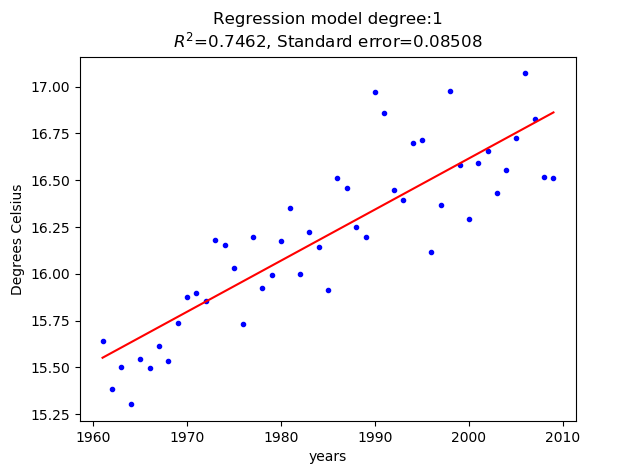
\includegraphics[width=0.6\linewidth]{fig/B.png}
\caption{问题B结果}
\end{figure}

Writeup回答
\begin{itemize}
	\item $R^2$变大了,拟合出来的直线依然呈上升趋势,且标准误差非常小,故同样能说明气候在变暖
	\item 因为拟合出来的直线呈上升趋势,且标准误差非常小
	\item 如果只用$3$个不同城市,随机性较大,故噪声很多,气温上升变化没有那么明显;
	如果使用$100$个不同城市,由于样本量足够,故噪声相对较小,应该能表现出明显的气温上升
	\item 噪声会变得更小(拟合误差变小),因为相近区域的气温差距一般不会太大
\end{itemize}

\subsection*{Part C:移动平均}
\verb'moving_average'主要问题在于求和范围的选择,特别要注意左边界条件。
利用Python的sliding技巧,可以很快写出以下代码。
\begin{lstlisting}
def moving_average(y, window_length):
    res = []
    for i in range(len(y)):
        if i < window_length:
            mean = pylab.mean(y[0:i+1])
        else:
            mean = pylab.mean(y[i-window_length+1:i+1])
        res.append(mean)
    return pylab.array(res)
\end{lstlisting}

\begin{figure}[H]
\centering
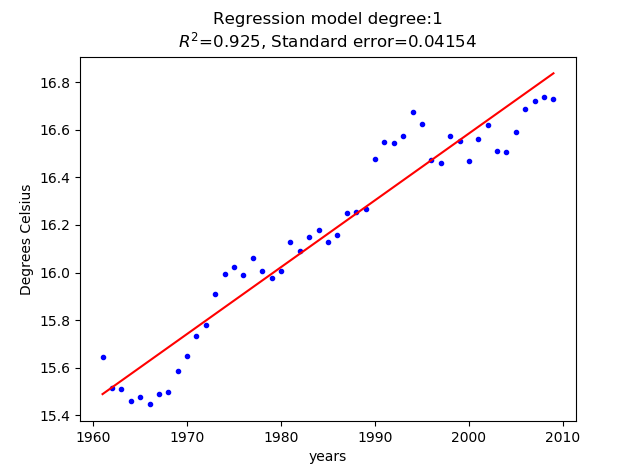
\includegraphics[width=0.6\linewidth]{fig/C.png}
\caption{问题C结果}
\end{figure}

Writeup回答
\begin{itemize}
	\item 拟合得更加好,点基本均匀分布在直线两侧,$R^2$变得更大,误差变得更小。
	\item 因为把邻近5年的数据都取了平均,进一步消除随机性带来的噪声,从而拟合得更好,数据点与直线间的距离更小。
\end{itemize}

\subsection*{Part D:预测未来}
\subsubsection{RMSE}
直接依照公式实现即可
\[RMSE=\sqrt{\frac{\sum_{i=1}^n(y_i-e_i)^2}{n}}\]

\verb'evaluate_models_on_testing'与\verb'evaluate_models_on_training'实现方式类似,仅仅是画图内容不同,因此这里不再赘述,详情请见代码。

\subsubsection{预测}
如下两个步骤,先生成更多模型(次数为1、2、20),然后用这些模型进行预测,并取移动平均。
\begin{lstlisting}
# Part D.2
# I. Generate more models
temperature = gen_cities_avg(climate,CITIES,years)
temperature_moving_avg = moving_average(temperature,5)
model = generate_models(years,temperature_moving_avg,[1,2,20])
evaluate_models_on_training(years,temperature_moving_avg,model)

# II. Predict the results
test_temperature = gen_cities_avg(climate,CITIES,test_years)
test_temperature_moving_avg = moving_average(test_temperature,5)
evaluate_models_on_testing(test_years,test_temperature_moving_avg,model)
\end{lstlisting}

\begin{figure}[H]
\centering
\begin{tabular}{cc}
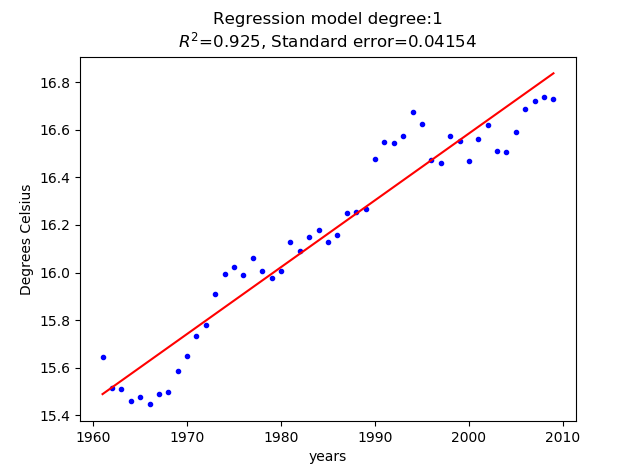
\includegraphics[width=0.5\linewidth]{fig/DI-1.png}&
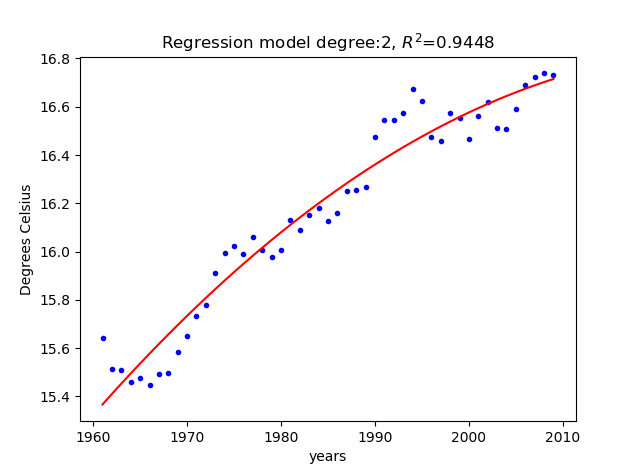
\includegraphics[width=0.5\linewidth]{fig/DI-2.png}\\
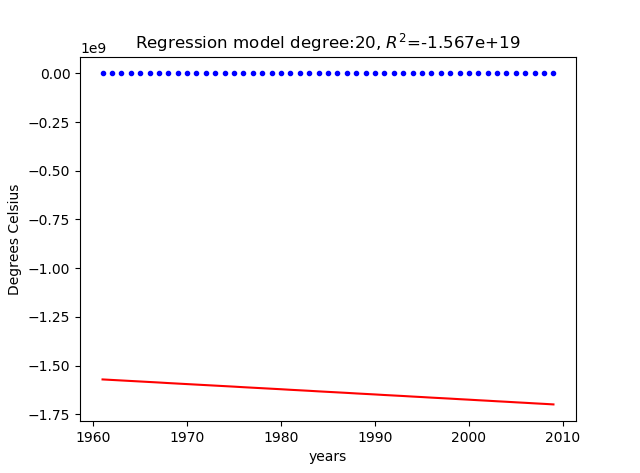
\includegraphics[width=0.5\linewidth]{fig/DI-3.png}
\end{tabular}
\caption{问题D.I结果}
\end{figure}

Writeup I回答
\begin{itemize}
	\item 度数为2的拟合效果最好,度数为20的拟合效果最差
	\item 度数为2的$R^2$最好,因为二次曲线能较好拟合数据,又不至于波动太大
	\item 度数为2的曲线拟合得最好,因为二次曲线度数刚刚好,能较好拟合数据,又不至于波动太大
\end{itemize}

\begin{figure}[H]
\centering
\begin{tabular}{cc}
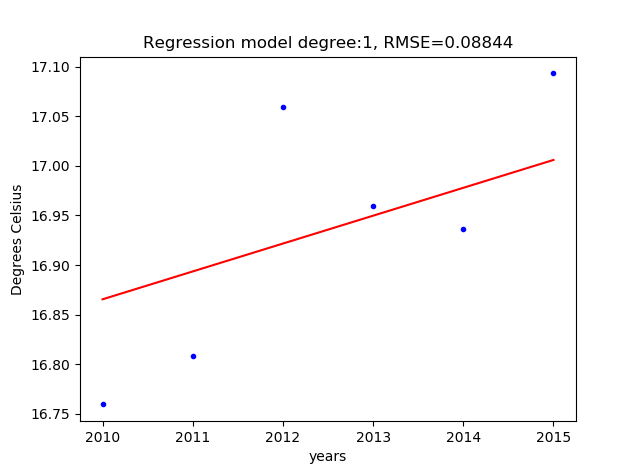
\includegraphics[width=0.5\linewidth]{fig/DII-1.png}&
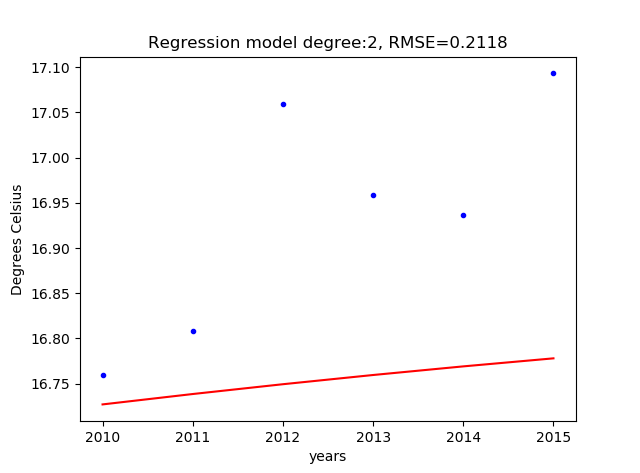
\includegraphics[width=0.5\linewidth]{fig/DII-2.png}\\
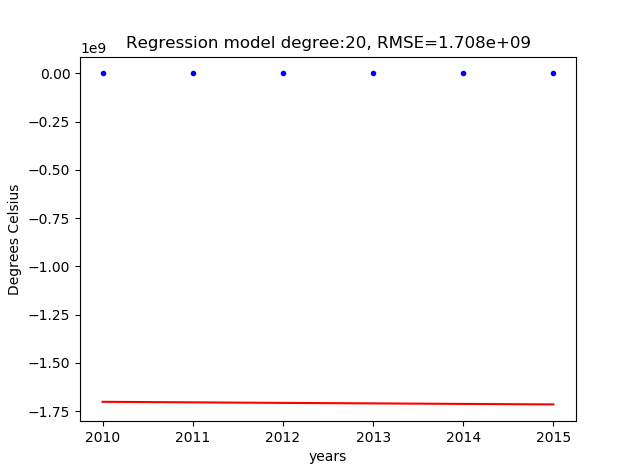
\includegraphics[width=0.5\linewidth]{fig/DII-3.png}
\end{tabular}
\caption{问题D.II结果}
\end{figure}

Writeup II回答
\begin{itemize}
	\item 度数为1的多项式预测效果比较合理,能使数据点均匀分布在两侧;
	度数为2和度数为20的多项式预测结果都偏低,所有实际数据点都在拟合曲线上方。
	关于RMSE,度数为1$<$度数为2$<<$度数为20。
	\item 线性预测得较好,度数为20的多项式最差。
	这与D.2.I的结果有点差异,二次曲线可能稍微有些过拟合,对未来的估计过为保守,故没有线性拟合的预测效果好。
	\item 见图\ref{fig:dii},预测结果将更加不稳定,但相比较之下,还是线性拟合的效果最好
\end{itemize}

\begin{figure}[H]
\centering
\begin{tabular}{cc}
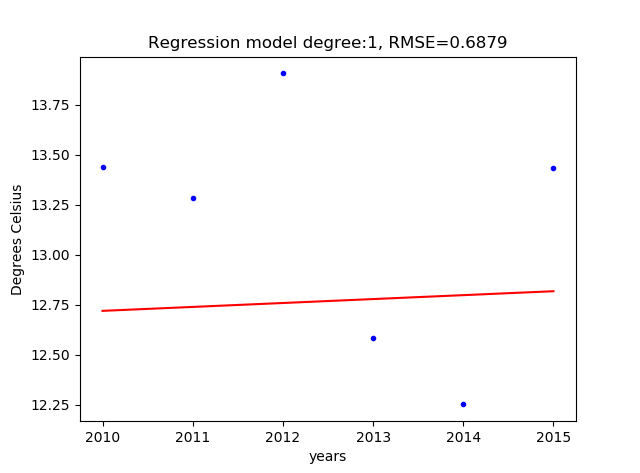
\includegraphics[width=0.5\linewidth]{fig/DIII-1.png}&
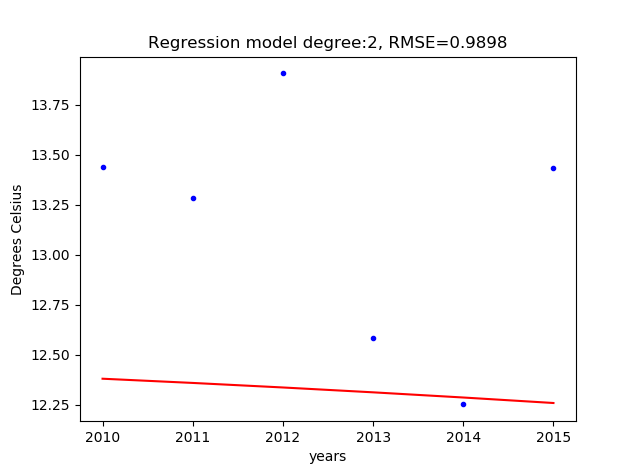
\includegraphics[width=0.5\linewidth]{fig/DIII-2.png}\\
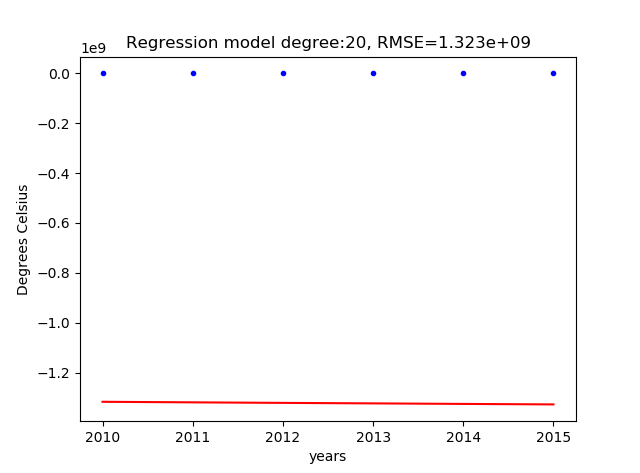
\includegraphics[width=0.5\linewidth]{fig/DIII-3.png}
\end{tabular}
\caption{问题D.II结果(用A.4.II数据拟合)}
\label{fig:dii}
\end{figure}

\subsection*{Part E:模拟极端气候}
\verb'gen_std_devs'与\verb'gen_cities_avg'的实施类似,关键是\verb'mean'的内容,这里应该对不同城市同一天的温度取平均,故\verb'axis=0'。
\begin{lstlisting}
def gen_std_devs(climate, multi_cities, years):
    res = []
    for year in years:
        temperature = []
        for city in multi_cities:
            temperature.append(climate.get_yearly_temp(city,year))
        daily_avg = pylab.mean(pylab.array(temperature),axis=0)
        res.append(pylab.std(daily_avg))
    return pylab.array(res)
\end{lstlisting}

\begin{figure}[H]
\centering
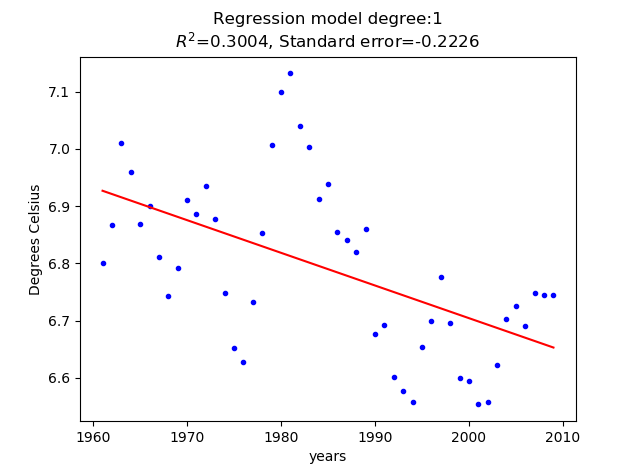
\includegraphics[width=0.6\linewidth]{fig/E.png}
\caption{问题E结果}
\end{figure}

Writeup回答
\begin{itemize}
	\item 气温的变化在变得越来越小
	\item 收集更多城市的数据;采用拟合程度更加好的模型,如埃尔米特插值等
\end{itemize}

\section{代码}
代码实施及注释请见附件\verb'ps5.py'。

\section{其他实验结果}
\label{sec:exp}
\begin{figure}[H]
\centering
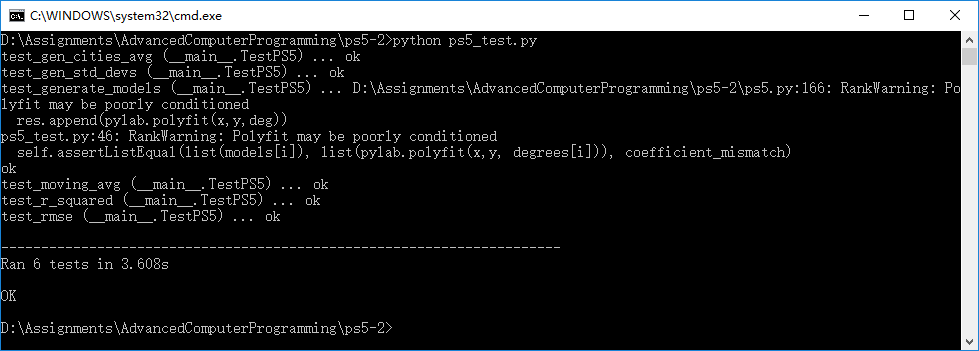
\includegraphics[width=\linewidth]{fig/test.PNG}
\caption{运行ps5\_tests.py的结果,可以看出所有测试样例通过}
\label{fig:test}
\end{figure}

\end{document}

% 实验提交内容
% 邮件主题,作业文件命名规范(学号、姓名) 学号+姓名+psX+vY
% 文档pdf格式(问题、求解思路、代码、注释、运行截图)
% 考虑健壮性、可读性
% 极端样例